\section{Constructive noise-free 4SID algorithm}

The 4SID algorithm is utilized to derive an estimated state-space model based on a truncated impulse response acquired from system measurements.

Beginning with a finite dataset of impulse response values, the algorithm operates under the assumption of a flawless, noise-free measurement of the impulse response. 
While the initial discussion centers on the algorithm's application to impulse response experiments for clarity, it's important to note its versatility to accommodate various types of input excitations.

The algorithm operates as follows:
\begin{enumerate}
    \item Construct the Hankel matrix in increasing order and assess its rank. 
        Cease increasing the order when encountering the first matrix lacking full rank.
        At this point,  the rank value denotes the system's order, denoted as $n$.
    \item Select $H_{n+1}$ (the first non-full rank matrix with a rank of $n$). 
        Decompose $H_{n+1}$  into two rectangular matrices of dimensions $(n+1) \times n$ and $n \times (n+1)$.
        The former matrix becomes $O_{n+1}$, while the latter becomes $R_{n+1}$, signifying the extended $(n+1)$ observability and reachability matrices, respectively.
    \item Derive $\hat{H}$, $\hat{G}$, and $\hat{F}$ from $O_{n+1}$ and $R_{n+1}$: 
        \[O_{n+1}=\begin{bmatrix} H \\ HF \\ HF^2 \\ \vdots \\ HF^{n-1} \\ HF^{n} \end{bmatrix} \qquad R_{n+1}=\begin{bmatrix} g \\ FG \\ F^2G \\ \vdots \\ F^{n-1}G \\ F^{n}G \end{bmatrix}\]
        Form this, $H$ and $G$ are directly extracted as the first row of $O_{n+1}$ and the first column of $R_{n+1}$, respectively. 
        To estimate $\hat{F}$, focus on $O_{n+1}$ (the same can be applied to $R_{n+1}$). 
        Formulate two submatrices, $O_1$ and $O_2$, by excluding the last and first rows of $O$, respectively:
        \[O_{1}=\begin{bmatrix} H \\ HF \\ HF^2 \\ \vdots \\ HF^{n-1} \end{bmatrix} \qquad O_{2}=\begin{bmatrix} HF \\ HF^2 \\ \vdots \\ HF^{n-1} \\ HF^{n} \end{bmatrix}\]
        Notably, $O_1$ and $O_2$ are square matrices owing to the shift invariance property.
        Consequently, $O_2=O_1\cdot F$.
        As $O_1$  is square and invertible (due to the full rank of $H_n$ with a row removed), $\hat{F}$ is determined as:
        \[\hat{F}=(O_1)^{-1}(O_2)\]
\end{enumerate}
It's important to note that we've derived the state space matrices by commencing with a noise-free impulse response experiment.

\begin{example}
    Consider a system represented by the following state-space matrices:
    \[F=\begin{bmatrix} \frac{1}{2} & 0 \\ 1 & \frac{1}{4} \end{bmatrix} \quad G=\begin{bmatrix} 1 \\ 0 \end{bmatrix} \quad H=\begin{bmatrix} 0 & 1 \end{bmatrix} \quad D=\begin{bmatrix} 0 \end{bmatrix}\]
    The system's order is determined by the order of matrix $F$, which is two.
    There's one input (as $G$ has one column) and one output (as $H$ has one row).
    The eigenvalues of $F$ $\left(\frac{1}{2} \text{ and } \frac{1}{4}\right)$ indicate asymptotic stability.

    The time-domain state-space equations are:
    \[\begin{cases}
        x_1(t+1)=\frac{1}{2}x_1+0x_2(t)+1u(t) \\ 
        x_2(t+1)=1x_1+\frac{1}{4}x_2(t)+0u(t) \\ 
        y(t)=0x_1(t)+1x_2(t)+0u(t)
    \end{cases}\]
    Which simplifies to:
    \[\begin{cases}
        x_1(t+1)=\frac{1}{2}x_1+u(t) \\ 
        x_2(t+1)=x_1+\frac{1}{4}x_2(t) \\ 
        y(t)=x_2(t)
    \end{cases}\]

    The block diagram of the system is:
    \begin{figure}[H]
        \centering
        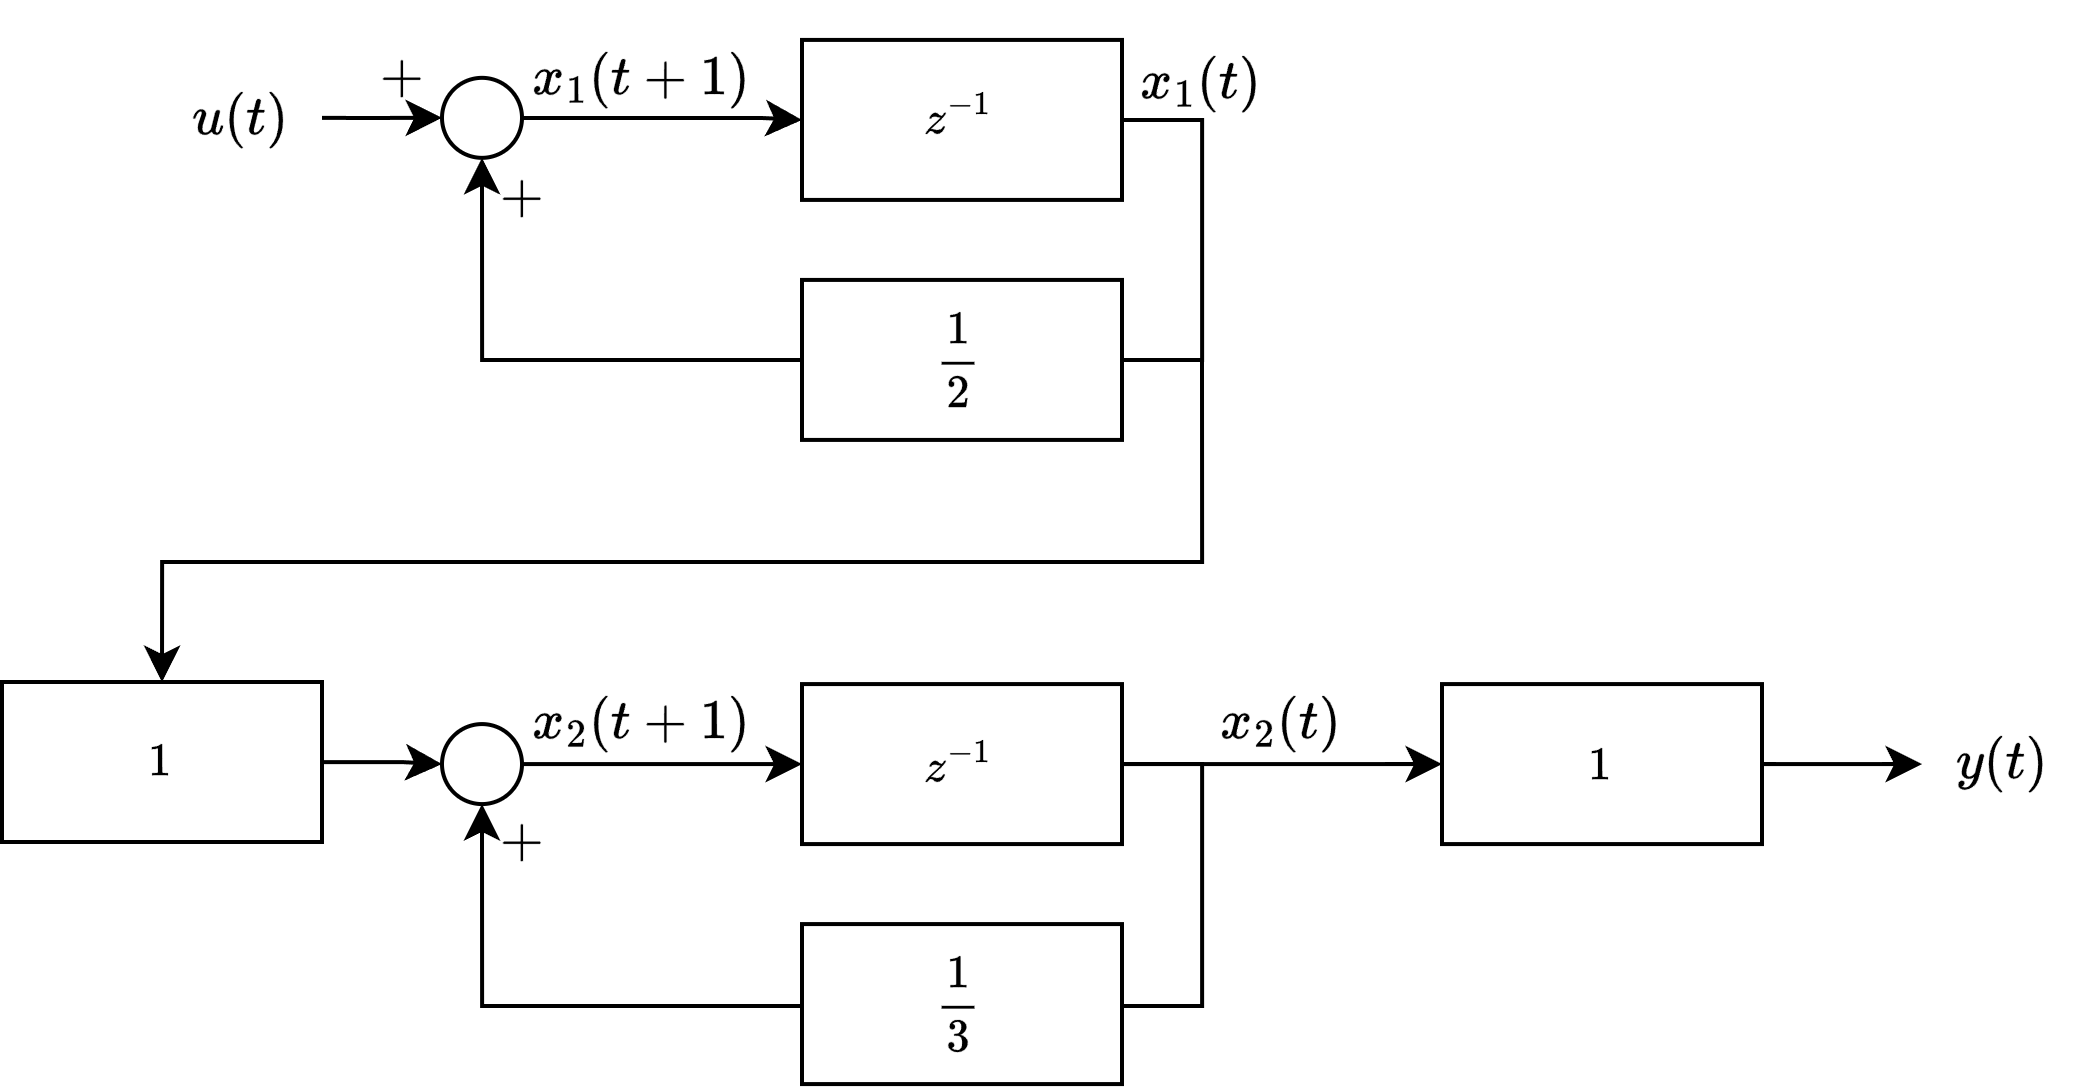
\includegraphics[width=0.6\linewidth]{images/block2.png}
    \end{figure}
    Visually, the system appears both controllable and observable. 
    Formally:
    \[O=\begin{bmatrix} H \\ HF \end{bmatrix}=\begin{bmatrix} 0 & 1 \\ 1 & \frac{1}{4} \end{bmatrix} \qquad R=\begin{bmatrix} G \\ FG \end{bmatrix}=\begin{bmatrix} 1 & \frac{1}{2} \\ 1 & 1 \end{bmatrix}\]
    Both $O$ and $R$ matrices have full rank, confirming controllability and observability.

    The extended observability and reachability matrices are computed as:
    \[O_3=\begin{bmatrix} H \\ HF \\ HF^2 \end{bmatrix}=\begin{bmatrix} 0 & 1 \\ 1 & \frac{1}{4} \\ \frac{3}{4} & \frac{1}{6} \end{bmatrix} \qquad R_3=\begin{bmatrix} G \\ FG \\ F^2G \end{bmatrix}=\begin{bmatrix} 1 & \frac{1}{2} & \frac{1}{4} \\ 1 & 1 & \frac{3}{4} \end{bmatrix}\]

    The transfer function from $u(t)$ to $y(t)$ can be computed in two ways:
    \begin{itemize}
        \item Direct manipulation of state-space equations:
            \[x_1(t+1)=\frac{1}{2}x_1+u(t)\rightarrow \dfrac{1}{z-\frac{1}{2}}u(t)\]
            \[x_2(t+1)=x_1+\frac{1}{4}x_2(t)\rightarrow zx_2(t)-\frac{1}{4}x_2(t)=\dfrac{1}{z-\frac{1}{2}}u(t)\rightarrow x_2(t)=\dfrac{1}{\left(z-\frac{1}{4}\right)\left(z-\frac{1}{2}\right)}u(t)\]
            Substituting the derived transfer functions into the last equation yields:
            \[y(t)=x_2(t)=\dfrac{1}{\left(z-\frac{1}{4}\right)\left(z-\frac{1}{2}\right)}u(t)\]
            Since this transfer function has two poles, which are identical to the system's eigenvalues, both representations contain the same information.
        \item Utilizing the direct formula, $W(z)=H\left(ZI-F\right)^{-1}H$, the result will be:
            \[W(z)=\dfrac{1}{\left(z-\frac{1}{4}\right)\left(z-\frac{1}{2}\right)}u(t)\]
    \end{itemize}

    We can also compute the impulse response representation up to instant five from the transfer function:
    \[W(z)=\dfrac{z^-2}{1-\frac{3}{4}z^{-1}+\frac{1}{8}z^{-2}}u(t)\]
    After performing five steps of long division, we obtain:
    \[E(z)=z^{-2}+\dfrac{3}{4}z^{-3}+\dfrac{7}{16}z^{-4}+\dfrac{15}{64}z^{-5}\]
    Thus, the corresponding impulse response is:
    \[\begin{cases}
        \omega(0)=0 \\
        \omega(1)=0 \\
        \omega(2)=1 \\
        \omega(3)=\frac{3}{4} \\
        \omega(4)=\frac{7}{16} \\
        \omega(5)=\frac{15}{64} \\
    \end{cases}\]

    The system order can also be found by incrementally building the Hankel matrix.
    The first matrix without full rank is $H_3$, indicating a system order of two.
\end{example}